\begin{figure*}[!htbp]

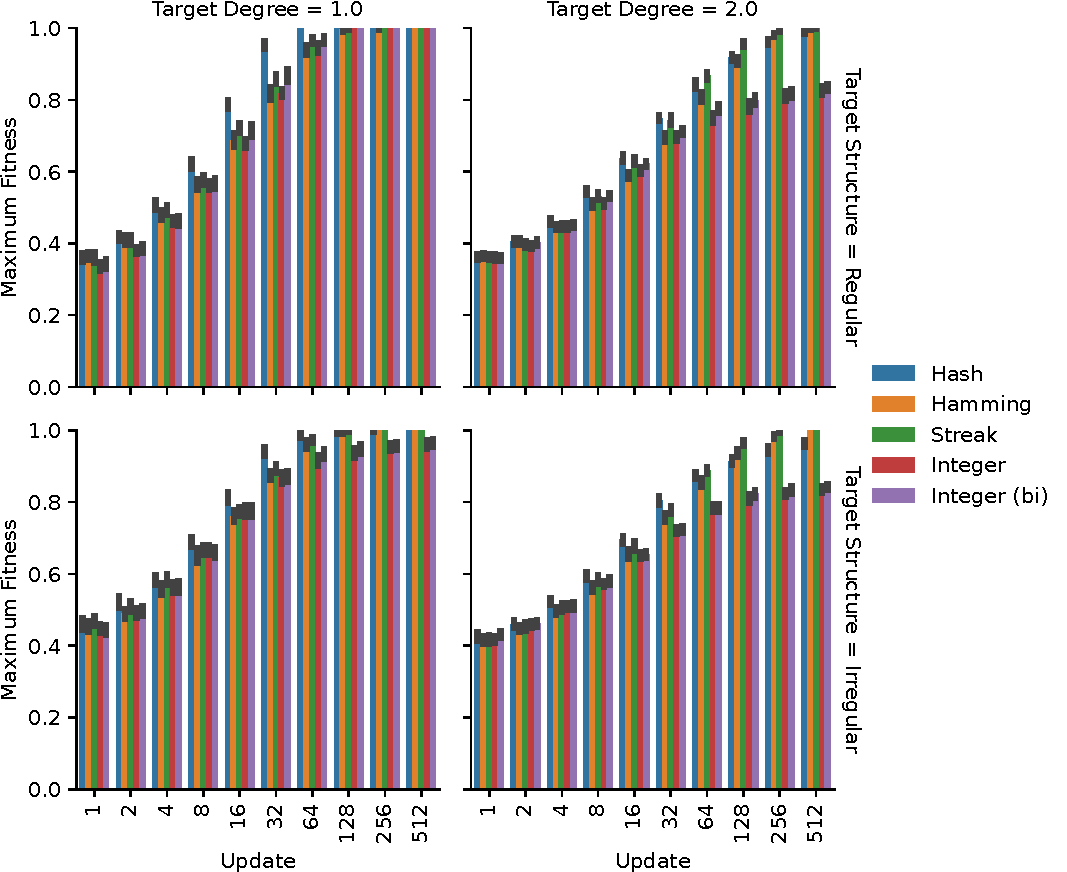
\includegraphics[width=\linewidth]{img/target_evolve/viz=max-fitness-bar+_data_hathash_hash=4c78832f20b46ffd+_script_fullcat_hash=c26c8688c31571c2+ext=}

\caption{
Trajectories of adaptive evolution for each tag-matching metric on the 32-vertex graph-matching task with randomly-initialized initial genomes.
Maximum fitness represents the best fitness value for any individual within a population.
Reported results use each metric's best-performing per-bit mutation rate.
(See Supplementary Figure \ref{fig:evolve_mutsweep} for survey showing how mutation rate affects adaptive evolution under each metric.)
Note log-scale x-axis.
Error bars represent bootstrapped 95\% confidence intervals across 50 replicate observations.
}
\label{fig:evolve_bests_bar}
\end{figure*}
